% Nama Kelompok : Kelompok 2
% Kelas : D4 TI 1A
% 1. Kadek Diva Krishna Murti (1174006)
% 2. Duvan Silalahi (1174011)
% 3. Oniwaldus (1174005)
% 4. Choirul Anam (1174004)
% 5. Sri Rahayu (1174015)
% 6. Ilham Habibi (1174028)

\documentclass{article}

\usepackage{amsmath}
\usepackage{textcomp}
\usepackage{graphicx}

\begin{document}



\section{Pengertian} 

\begin{figure}[ht]
\centerline{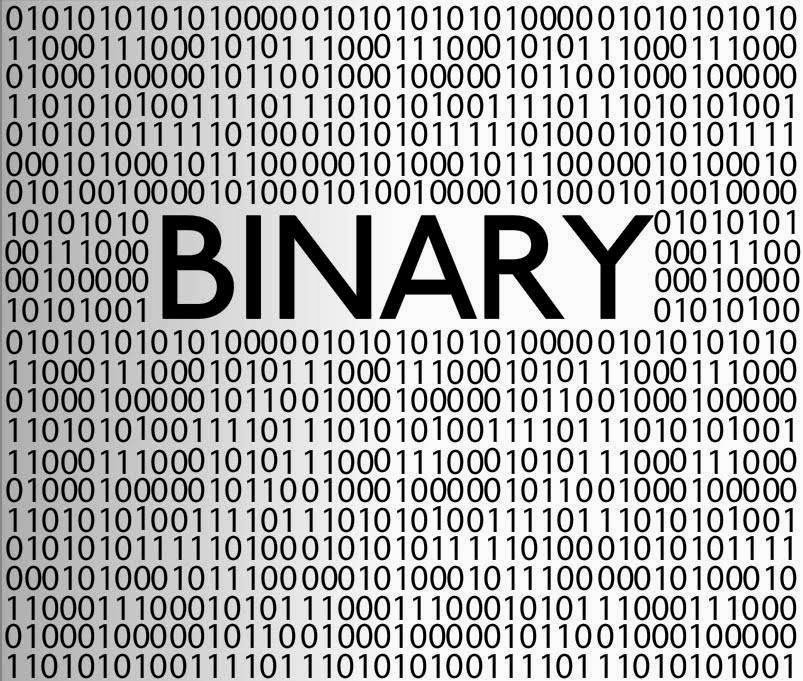
\includegraphics[width=0.4\textwidth]{../figures/biner.jpg}}
\caption{Sistem bilangan biner.}
\label{biner}
\end{figure}

Sejak pertama kali komputer elektronik digunakan, komputer tersebut telah beroperasi dengan menggunakan sistem bilangan biner, yaitu bilangan berbasis dua pada sistem bilangan. Semua kode program dan data pada komputer disimpan serta dimanipulasi dalam format biner yang merupakan kode - kode mesin komputer. Sehingga semua perhitungan – perhitungan yang diolah oleh computer tersebut menggunakan aritmatika biner yang hasilnya berupa bilangan hanya memiliki dua kemungkinan nilai, yaitu 0 dan 1. 

\begin{figure}[ht]
\centerline{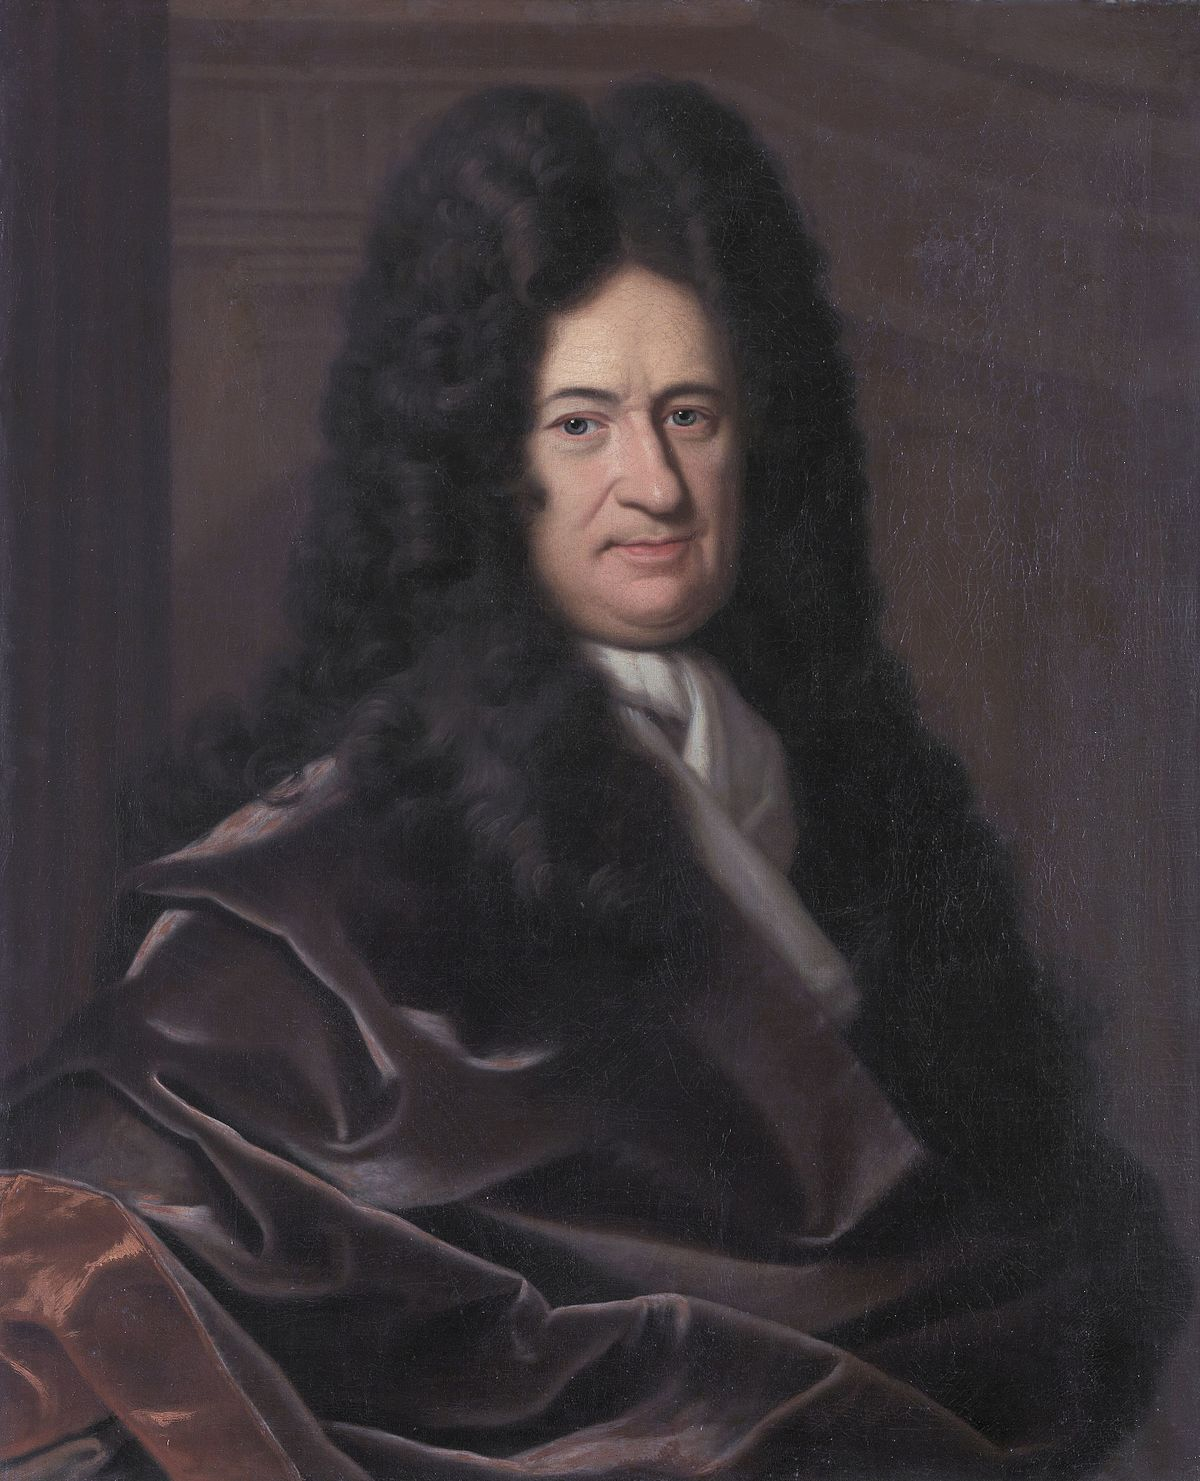
\includegraphics[width=0.4\textwidth]{../figures/gwl.jpg}}
\caption{Penemu sistem bilangan biner.}
\label{gwl}
\end{figure}

Dikutip dari \cite{hutahaean2015konsep} bilangan biner \ref{biner} atau bilangan berbasis dua atau binary dalam Bahasa Inggris merupakan sebuah penulisan bilangan di mana bilangan – bilangan tersebut hanya menggunakan dua angka, yaitu 0 dan 1. Tidak seperti bilangan desimal yang merupakan sistem bilangan berbasis 10, sistem bilangan biner berbasis 2. bilangan biner digunakan untuk informasi biner dan juga satuan ukuran besarnya data. Sistem bilangan biner modern ditemukan oleh Gottfried Wilhelm Leibniz \ref{gwl} pada abad ke-17. Sistem bilangan ini merupakan dasar dari semua sistem bilangan berbasis digital. Dari sistem biner , kita dapat mengkonversinya ke sistem bilangan Oktal atau Hexadesimal. Sistem ini juga dapat kita sebut dengan istilah bit atau Binary Digit atau dalam arsitektur elektronik biasa disebut sebagai digital logic.. 

Pengelompokan biner dalam komputer selalu berjumlah 8, dengan istilah 1 Byte atau bita. Dalam istilah komputer, 1 Byte = 8 bit. Kode-kode rancang bangun sistem bilangan berbasis 10, sistem bilangan biner berbasis 2. Bilangan biner digunakan untuk informasi biner dan juga satuan ukuran besarnya data.

Sistem bilangan ini merupakan dasar dari semua sistem bilangan berbasis digital. Dari sistem biner, kita dapat mengkonversinya ke sistem bilangan Oktal atau Hexadesimal. Sistem ini juga dapat kita sebut dengan istilah bit atau Binary Digit atau dalam arsitektur elektronik biasa disebut sebagai digital logic. Pengelompokan biner dalam komputer selalu berjumlah 8, dengan istilah 1 Byte atau bita. Dalam istilah komputer, 1 Byte = 8 bit. Kode-kode rancang bangun komputer seperti ASCII, American Standard Code for Information Interchange menggunakan sistem pengkodean 1 Byte.

Setiap digit pada bilangan biner mewakili pangkat pada angka 2 yang terus meningkat dari kanan ke kiri, Digit yang paling kanan mewakili 2 pangkat 0 ($2^0$). digit selanjutnya mewakili 2 pangkat 1 ($2^1$), selanjutnya lagi mewakili mewakili 2 pangkat 2 ($2^2$), dan seterusnya. Bilangan desimal 0 diwakili dengan bilangan biner '0', begitu juga dengan bilangan desimal 1 diwakili dengan bilangan biner '1'. Kedua bilangan 1 dan 0 tersebut tidak berubah. Bilangan desimal 2 diwakili sebagai bilangan biner '10', 3 sebagai '11', 4 sebagai '100', 5 sebagai '101', dan seterusnya.

Dalam sistem komunikasi digital modern, dimana data ditransmisikan dalam bentuk bit-bit biner, dibutuhkan sistem yang tahan terhadap noise yang terdapat di kanal transmisi sehingga data yang ditransmisikan tersebut dapat diterima dengan benar. Kesalahan dalam pengiriman atau penerimaan data merupakan permasalahan yang mendasar yang memberikan dampak yang sangat signifikan pada sistem komunikasi.Biner yang biasa dipakai itu ada 8 digit angka dan cuma berisikan angka 1 dan 0, tidak ada angka lainnya.
Posisi sebuah angka dalam bilangn biner atau bilangan basis dua akan menentukan berapa bobot nilainya. Posisi paling depan (kiri) sebuah bilangan memiliki nilai yang paling besar sehingga disebut sebagai MSB (Most Significant Bit), dan posisi paling belakang (kanan) sebuah bilangan memiliki nilai yang paling kecil sehingga disebut sebagai LSB (Leased Significant Bit). Berikut ini adalah contoh representasi dari bilangan biner atau bilangan berbasis dua : 
$10110_2$ = 1 x $2^4$ + 0 x $2^3$ + 1 x $2^2$ + 1 x $2^1$ + 0 x $2^0$ = $22_{10}$

\subsection{Bilangan Biner}
Sebagai contoh dari bilangan desimal, untuk angka 157 : $157_{(10)}$ = (1 x 100) + (5 x 10) + (7 x 1) 
Perhatikan! Bilangan desimal ini sering juga disebut dengan basis 10. Hal ini dikarenakan perpangkatan 10 yang didapat dari 100, 101, 102, dst. 
\subsubsection{Mengenal Konsep Bilangan Biner dan Desimal}
Perbedaan paling mendasar dari metode bilangan biner dan bilangan desimal terletak pada jumlah dari basisnya. Jika desimal berbasis 10(X10) berpangkatkan 10x, maka untuk bilangan biner berbasiskan 2 (x2) menggunakan perpangkatan 2x. Sederhananya perhatikan contoh dibawah ini!\\
Untuk Desimal:\\
$14_{(10)}$=(1x$^1$) + (4 x $10^0$)\\
=10 + 4\\
=14\\
Untuk Biner: \\
$1110_{(2)}$ = (1 x 23) + (1 x 22) + (1 x 21) + (0 x 20)\\
 = 8 + 4 + 2 + 0\\
 = 14\\

Bentuk umum dari bilangan biner dan bilangan desimal bisa dilihat pada tabel \ref{table:binerdesimal}. 

\begin{table}[h!]
\centering
\begin{tabular}{ |c|c|c|c|c|c|c|c|c|c| } 
\hline
Biner & 1 & 1 & 1 & 1 & 1 & 1 & 1 & 1 & 11111111 \\ 
\hline
Desimal & 128 & 64 & 32 & 16 & 8 & 4 & 2 & 1 & 255 \\ 
\hline
Pangkat & $2^7$ & $2^6$ & $2^5$ & $2^4$ & $2^3$ & $2^2$ & $2^1$ & $2^0$ & $X^{1-7}$ \\ 
\hline
\end{tabular}
\caption{Tabel bentuk umum dari bilangan biner dan bilangan desimal}
\label{table:binerdesimal}
\end{table}

Sekarang kita balik lagi ke contoh soal di atas! Darimana kita dapatkan angka desimal 14(10) menjadi angka biner 1110(2)? 
Mari kita lihat lagi pada bentuk umumnya pada tabel \ref{table:contoh1}!

\begin{table}[h!]
\centering
\begin{tabular}{ |c|c|c|c|c|c|c|c|c|c| } 
\hline
Biner & 0 & 0 & 0 & 0 & 1 & 1 & 1 & 0 & 00001110 \\ 
\hline
Desimal & 0 & 0 & 0 & 0 & 8 & 4 & 2 & 0 & 14 \\ 
\hline
Pangkat & $2^7$ & $2^6$ & $2^5$ & $2^4$ & $2^3$ & $2^2$ & $2^1$ & $2^0$ & $X^{1-7}$ \\ 
\hline
\end{tabular}
\caption{Tabel contoh biner ke desimal.}
\label{table:contoh1}
\end{table}

Mari kita telusuri perlahan-lahan!

\begin{enumerate}
\item Pertama sekali, kita jumlahkan angka pada desimal sehingga menjadi 14. anda lihat angka - angka yang menghasilkan angka 14 adalah 8, 4, dan 2!
\item Untuk angka-angka yang membentuk angka 14 (lihat angka yang diarsir), diberi tanda biner “1”, selebihnya diberi tanda “0”.
\item Sehingga kalau dibaca dari kanan, angka desimal 14 akan menjadi 00001110 (terkadang dibaca 1110) pada angka biner nya.
\end{enumerate}


\subsubsection{Mengubah Angka Biner ke Desimal}
Perhatikan contoh! 

\begin{enumerate}
\item 11001101(2) 

\begin{table}[h!]
\centering
\begin{tabular}{ |c|c|c|c|c|c|c|c|c|c| } 
\hline
Biner & 1 & 1 & 0 & 0 & 1 & 1 & 0 & 1 & 11001101 \\ 
\hline
Desimal & 128 & 64 & 0 & 0 & 8 & 4 & 0 & 1 & 205 \\ 
\hline
Pangkat & $2^7$ & $2^6$ & $2^5$ & $2^4$ & $2^3$ & $2^2$ & $2^1$ & $2^0$ & $X^{1-7}$ \\ 
\hline
\end{tabular}
\caption{Tabel contoh biner ke desimal.}
\label{table:contoh2}
\end{table}

Note:

\begin{itemize}
\item Angka desimal 205 didapat dari penjumlahan angka yang di arsir (128+64+8+4+1)
\item Setiap biner yang bertanda “1” akan dihitung, sementara biner yang bertanda “0” tidak dihitung, alias “0” juga.
\end{itemize}

\item 00111100(2) 

\begin{table}[h!]
\centering
\begin{tabular}{ |c|c|c|c|c|c|c|c|c|c| } 
\hline
Biner & 0 & 0 & 1 & 1 & 1 & 1 & 0 & 0 & 00111100 \\ 
\hline
Desimal & 0 & 0 & 32 & 16 & 8 & 4 & 0 & 0 & 60 \\ 
\hline
Pangkat & $2^7$ & $2^6$ & $2^5$ & $2^4$ & $2^3$ & $2^2$ & $2^1$ & $2^0$ & $X^{1-7}$ \\ 
\hline
\end{tabular}
\caption{Tabel contoh biner ke desimal.}
\label{table:contoh2}
\end{table}

Note:
\begin{itemize}
\item Angka desimal 60 didapat dari penjumlahan angka yang di arsir (32+16+8+4)
\item Setiap biner yang bertanda "1" akan dihitung, sementara biner yang bertanda "0" tidak dihitung, alias "0" juga.
\end{itemize}

\subsubsection {Mengubah Angka Desimal ke Biner} 
Untuk mengubah angka desimal menjadi angka biner digunakan metode pembagian dengan angka 2 sambil memperhatikan sisanya. 
Perhatikan contohnya! 
\begin{enumerate}
\item 205(10)\\
205 : 2 = 102 sisa 1\\ 
102 : 2 = 51 sisa 0 \\
51 : 2 = 25 sisa 1\\
25 : 2 = 12 sisa 1 \\
12 : 2 = 6 sisa 0 \\
6 : 2 = 3 sisa 0 \\
3 : 2 = 1 sisa 1 \\
1 \textrightarrow sebagai sisa akhir "1"\\
Note :
Untuk menuliskan notasi binernya, pembacaan dilakukan dari bawah yang berarti 11001101(2) 

\item 60(10)\\
60 : 2 = 30 sisa 0\\ 
30 : 2 = 15 sisa 0 \\
15 : 2 = 7 sisa 1 \\
7 : 2 = 3 sisa 1 \\
3 : 2 = 1 sisa 1 \\
1 \textrightarrow sebagai sisa akhir "1"\\
Note :
Dibaca dari bawah menjadi 111100(2) atau lazimnya dituliskan dengan 00111100(2). Ingat bentuk umumnnya mengacu untuk 8 digit! Kalau 111100 (ini 6 digit) menjadi 00111100 (ini sudah 8 digit). 

\end{enumerate}

\subsection{Aritmatika Biner}

Pada bagian ini akan membahas penjumlahan dan pengurangan biner. Perkalian biner adalah pengulangan dari penjumlahan; dan juga akan membahas pengurangan biner berdasarkan ide atau gagasan komplemen.

\begin{enumerate}

\item Penjumlahan Biner

Penjumlahan biner tidak begitu beda jauh dengan penjumlahan desimal. Perhatikan contoh penjumlahan desimal antara 167 dan 235.
1 \textrightarrow 7+5 = 12, tulis "2" di bawah dan angkat "1" ke atas! \\
167 \\
235 \\
------ + \\
402 \\

Seperti bilangan desimal, bilangan biner juga dijumlahkan dengan cara yang sama. Pertama-tama yang harus dicermati adalah aturan pasangan digit biner berikut:
0 + 0 = 0 \\
0 + 1 = 1 \\
1 + 1 = 0 \textrightarrow dan menyimpan 1 \\

sebagai catatan bahwa jumlah dua yang terakhir adalah : \\
1 + 1 + 1 = 1 \textrightarrow dengan menyimpan 1 \\

Dengan hanya menggunakan penjumlahan penjumlahan di atas, kita dapat melakukan penjumlahan biner seperti ditunjukkan di bawah ini: \\
11111 \textrightarrow “simpanan 1” ingat kembali aturan di atas! \\
01011011 \textrightarrow bilangan biner untuk 91 \\
01001110 \textrightarrow bilangan biner untuk 78 \\
------------ + \\
10101001 \textrightarrow Jumlah dari 91 + 78 = 169 \\

Silahkan pelajari aturan-aturan pasangan digit biner yang telah disebutkan di atas! Contoh penjumlahan biner yang terdiri dari 5 bilangan! \\
11101 bilangan 1) \\
10110 bilangan 2) \\
1100 bilangan 3) \\
11011 bilangan 4) \\
1001 bilangan 5) \\
-------- + \\

Untuk menjumlahkannya, kita hitung berdasarkan aturan yang berlaku, dan untuk lebih mudahnya perhitungan dilakukan bertahap. \\
11101 bilangan 1) \\
10110 bilangan 2) \\
-------- + \\
110011
1100 bilangan 3) \\
-------- + \\
111111 \\
11011 bilangan 4) \\ 
-------- + \\
011010 \\
1001 bilangan 5) \\ 
-------- + \\
1100011 \textrightarrow Jumlah Akhir. \\
Berapakah bilangan desimal? \\
Sekarang coba tentukan berapakah bilangan 1,2,3,4 dan 5! Apakah memang perhitungan di atas sudah benar? \\

\item Pengurangan Biner

Pengurangan bilangan desimal 73426 – 9185 akan menghasilkan: \\
73426 \textrightarrow lihat! Angka 7 dan angka 4 dikurangi dengan 1 \\
9185 \textrightarrow digit desimal pengurang. \\
--------- - \\
64241 \textrightarrow Hasil pengurangan akhir. \\
Bentuk Umum pengurangan : \\
0 – 0 = 0 \\
1 – 0 = 1 \\
1 – 1 = 0 \\



0 – 1 = 1 \textrightarrow dengan meminjam „1‟ dari digit disebelah kirinya! \\ 
Untuk pengurangan biner dapat dilakukan dengan cara yang sama. Coba perhatikan bentuk pengurangan berikut: \\
1111011 \textrightarrow desimal 123 \\
101001 \textrightarrow desimal 41 \\
--------- - \\
1010010 \textrightarrow desimal 82 \\
Pada contoh di atas tidak terjadi “konsep peminjaman”. Perhatikan contoh berikut! \\





0 \textrightarrow kolom ke-3 sudah menjadi „0‟, sudah dipinjam! \\
111101 \textrightarrow desimal 61 \\
10010 \textrightarrow desimal 18 \\
------------ - \\
101011 \textrightarrow Hasil pengurangan akhir 43. \\

Pada soal yang kedua ini kita pinjam „1‟ dari kolom 3, karena ada selisih 0-1 pada kolom ke-2. Lihat Bentuk Umum! \\





7999 \textrightarrow hasil pinjaman \\
800046 \\
397261 \\
--------- - \\
402705 \\
Sebagai contoh pengurangan bilangan biner 110001 – 1010 akan diperoleh hasil sebagai berikut: \\
1100101 \\
1010 \\
---------- - \\
100111 \\

\item Komplomen

Salah satu metoda yang dipergunakan dalam pengurangan pada komputer yang ditransformasikan menjadi penjumlahan dengan menggunakan minusradiks komplemen satu atau 




komplemen radiks. Pertama-tama kita bahas komplemen di dalam sistem desimal, dimana komplemen-komplemen tersebut secara berurutan disebut dengan komplemen sembilan dan komplemen sepuluh (komplemen di dalam sistem biner disebut dengan komplemen satu dan komplemen dua). Sekarang yang paling penting adalah menanamkan prinsip ini: \\
“Komplemen sembilan dari bilangan desimal diperoleh dengan mengurangkan masing-masing 




digit desimal tersebut ke bilangan 9, sedangkan komplemen sepuluh adalah komplemen sembilan ditambah 1” \\
Lihat contoh nyatanya! \\
Bilangan Desimal 123 651 914 \\
Komplemen Sembilan 876 348 085 \\ 
Komplemen Sepuluh 877 349 086 \textrightarrow ditambah dengan 1! \\
Perhatikan hubungan diantara bilangan dan komplemennya adalah simetris. Jadi, dengan memperhatikan contoh di atas, komplemen 9 dari 123 adalah 876 dengan simple menjadikan jumlahnya = 9 (1+8=9, 2+7=9, 3+6=9)! \\
Sementara komplemen 10 didapat dengan menambahkan 1 pada komplemen 9, berarti 876+1=877. \\
Pengurangan desimal dapat dilaksanakan dengan penjumlahan komplemen sembilan plus satu, atau penjumlahan dari komplemen sepuluh. \\

\begin{center}
\begin{tabular}{ c c c }
893 & 893 & 893 \\ 
321 & 678 (komp. 9) & 679 (komp. 10) \\
----- - & ----- + & ----- + \\
572 & 1571 & 1572 \\
& 1 & \\
& ----- - & \\
& 572 \textrightarrow angka 1 dihilangkan& \\
\end{tabular}
\end{center}

\end{enumerate}
Analogi yang bisa diambil dari perhitungan komplemen di atas adalah, komplemen satu dari bilangan biner diperoleh dengan jalan mengurangkan masing masing digit biner tersebut ke bilangan 1, atau dengan bahasa sederhananya mengubah masing-masing 0 menjadi 1 atau sebaliknya mengubah masing-masing 1 menjadi 0. Sedangkan komplemen dua adalah satu plus satu. \\
Perhatikan Contoh. \\
Bilangan Biner 110011 101010 011100 \\
Komplemen Satu 001100 010101 100011 \\
Komplemen Dua 001101 010110 100100 \\

Pengurangan biner 110001 – 1010 akan kita telaah pada contoh di bawah ini! \\
110001 110001 110001 \\
001010 110101 110110 \\
--------- - -------- + --------- + \\
100111 100111 1100111 dihilangkan! \\
Alasan teoritis mengapa cara komplemen ini dilakukan, dapat dijelaskan dengan memperhatikan sebuah speedometer mobil/motor dengan empat digit sedang membaca nol. \\



%Lanjutkan diatas tulisan ini
\end{enumerate}
\end{document}